\chapter{Writing Qonverter}
Libraries and compiler are selected. Let's think about application. Let's assume we need to write simple and easy-to-use calculator application, which should run on Windows and Linux. We already know something about Qt and we are able to seek for needed information in \citep{various:qtdoc}. Qonverter should run in single window mode but we may eventually need to hide it into tray area. So tray icon functionality has to be provided.

\begin{fdocextra}
Use source code of Qonverter tu understand this part of the book. Source code is commented and this part of the book is (intentionally) just collection of hints on how to build your own Qt application.
\end{fdocextra}

Qonverter should be translated to English (as it is globally spoken language) and Czech which is the native language of the author of this book. Qonverter should fit into desktop environments so native icon themes with fall-back theme should be used. Installation of Qonverter should be as easy as possible. This means simple ZIP archive for Windows and native package for Linux distributions. More specific feature list for Qonverter could look like this one:
\begin{itemize}
\item use muParserX as mathematical core,
\item offer unit and currency converters,
\item support on-line currency rates synchronization for currency converter,
\item allow conversions of mathematical formulas for unit converter (This means that for example formula $5+7$ is computed first and result is then converted as needed.),
\item calculator is simple,
\item most used functions are accessible via calculator keypad,
\item input text box for mathematical formulas in calculator is multi-line,
\item language of the application can be switched manually,
\item free software license is used,
\item user can define variables,
\item many built-in constants,
\item application depends only on Qt and muParserX.
\end{itemize}

These are primary goals. Optional goals appear during the course of development.

\section{Qonverter structure}
Qonverter application consists of two main parts:
\begin{description}
\item[CORE] \hfill \\
Is based on muParserX library and is responsible for providing results of input formulas. Logic of currency (unit) converter is separated into core too. Core doesn't depend on graphical interface of the application.
\item[\fdocabbrevref{GUI}] \hfill \\
Forms visual part of the application and provides user with main application window and switchable tray icon.
\end{description}

\section{Programming application core}
We need to wrap muParserX library and make reasonable subset of its functionality available through Qt-friendly interface. This is done by\fdocinlinecode{cpp}{!}{Calculator} class. One of its main goals is to provide tools for numerical computations. muParserX library originally does computations via\fdocinlinecode{cpp}{!}{ParserX} class. Its typical usage is shown in \autoref{listing:parser}. We see that we created\fdocinlinecode{cpp}{!}{ParserX} instance and set the expression. Then we tried to evaluate it. Any exception is caught and error description is written to the standard output.

\begin{fdoccode}{cpp}{listing:parser}{Basic ParserX class usage}
ParserX m_parser;
m_parser.SetExpr("5+7");

Value result;
try {
	// Evaluate the expression.
	result = m_parser.Eval();
}
catch (ParserError &e) {
	qDebug("Error occurred.");
}
// The 'result' variable contains result of computation.
\end{fdoccode}

\indent\fdocinlinecode{cpp}{!}{Calculator} class should provide enhanced approach for numerical computations and it does as it offers method\fdocinlinecode{cpp}{!}{void calculateExpression(Calculator::CallerFunction function, QString expression)} method. This method takes any mathematical expression in textual form and identification of target function.

Note that numerical computations may take some time. Thus, we need to calculate expressions asynchronously.

\indent\fdocinlinecode{cpp}{!}{Calculator} class will be used in the \textit{singleton} pattern and will be separated in its own thread by\fdocinlinecode{cpp}{!}{CalculatorWrapper} class which manages\fdocinlinecode{cpp}{!}{Calculator} singleton instance. This class basically just starts the thread with calculator and quits it if needed (\autoref{listing:thrq}).

\begin{fdoccode}{cpp}{listing:thrq}{Running calculator in separated thread}
// CalculatorWrapper constructor.
CalculatorWrapper::CalculatorWrapper(QObject *parent) : QObject(parent) {
  // Create calculator.
  m_calculator = new Calculator();

  // Create separate thread for calculator.
  m_thread = new QThread();

  // Prepare calculator for usage in separate thread.
  m_calculator->moveToThread(m_thread);

  // Connect thread to calculator.
  connect(m_thread, &QThread::started, m_calculator, &Calculator::initialize);
  connect(m_thread, &QThread::finished, m_thread, &QThread::deleteLater);
}

// CalculatorWrapper destructor.
CalculatorWrapper::~CalculatorWrapper() {
  qDebug("Deleting calculator wrapper.");

  m_thread->quit();
  m_thread->wait(1000);

  delete m_calculator;
}

CalculatorWrapper &CalculatorWrapper::getInstance() {
  if (s_instance.isNull()) {
    s_instance.reset(new CalculatorWrapper());
    s_instance.data()->m_thread->start();
  }

  return *s_instance;
}
\end{fdoccode}

Qonverter builds on muParserX in aspect of variables, functions and constants. Qonverter wraps all these entities in single structure called\fdocinlinecode{cpp}{!}{MemoryPlace}. It holds information about the actual type of underlying entity.
\begin{lstlisting}[firstnumber=1,language=cpp]
enum Type {
  CONSTANT = 0,
  IMPLICIT_VARIABLE = 1,
  EXPLICIT_VARIABLE = 2,
  SPECIAL_VARIABLE = 3,
  FUNCTION = 4
};
\end{lstlisting}
Structure\fdocinlinecode{cpp}{!}{MemoryPlace} (\autoref{listing:memoryplaceh}) defines properties used for constants, variables or functions, including name and description.\fdocinlinecode{cpp}{!}{MemoryPlace} can encapsulate these kinds of entities:
\begin{description}
\item[CONSTANTS] \hfill \\
Constants are named values. Values of constants do not change. Constants are special numbers which are interesting in some way and are used extensively in mathematical computations.
\item[FUNCTIONS] \hfill \\
Functions are stored as\fdocinlinecode{cpp}{!}{MemoryPlace} instances too. Each function is described by its name and description.
\item[VARIABLES] \hfill \\
We can divide variables into three categories:
\begin{enumerate}
\item IMPLICITLY-CREATED VARIABLES \\[3px]
Those are created during evaluation of mathematical expression by calculator engine.
\item EXPLICITLY-CREATED VARIABLES \\[3px]
Explicitly-created variables are defined manually by application user.
\item CRITICAL VARIABLES \\[3px]
Critical variables are just ordinary variables with one exception\,--\,they cannot be deleted. They are used for storing last two successfully calculated results (variables\fdocinlinecode{cpp}{!}{ans} and\fdocinlinecode{cpp}{!}{ansx}) and for main memory variable\fdocinlinecode{cpp}{!}{m}.
\end{enumerate}
\end{description}

\begin{fdoccode}{cpp}{listing:memoryplaceh}{Declaration of MemoryPlace class}
// Represents entity which as able to hold value.
// This includes calculator variables and constants.
struct MemoryPlace {
    QString m_name;
    QString m_description;
    Value *m_value;
    Type m_type;

    // This is used only by variables, each constant has m_variable equal to nullptr.
    // So there is way to distinguish variables from constants.
    Variable *m_variable;

    // Constructs "empty" variable.
    // This constructor is used for constructing
    // "shallow" clones of implicitly-created variables.
    MemoryPlace(const QString &name);

    // Creates new variable or constant
    MemoryPlace(const QString &name, const QString &description,
                const Value &value, const Type &type);

    // Destructor.
    ~MemoryPlace();
};
\end{fdoccode}
Declaration of this class is straighforward but let's take a look at destructor implementation (\autoref{listing:memoryplaceh2}).

\begin{fdoccode}{cpp}{listing:memoryplaceh2}{MemoryPlace class destructor}
MemoryPlace::~MemoryPlace() {
  // Free resources of this object if:
  if (m_type == CONSTANT || m_type == FUNCTION) {
    delete m_value;
    qDebug("Constant '%s' deleted.", qPrintable(m_name));
  }
  else if (m_type == EXPLICIT_VARIABLE || m_type == SPECIAL_VARIABLE) {
    delete m_value;
    delete m_variable;
    qDebug("Variable '%s' deleted.", qPrintable(m_name));
  }
  else {
    qDebug("Implicitly-created variable '%s' deleted.", qPrintable(m_name));
  }
}
\end{fdoccode}
We see that destructor looks complicated because freeing of\fdocinlinecode{cpp}{!}{m_value} and\fdocinlinecode{cpp}{!}{m_variable} properties is conditional. In fact, constants and functions do not use\fdocinlinecode{cpp}{!}{m_variable} property which is not freed in those cases. Also note that nothing is freed from the memory in case of implicit variables. Properties\fdocinlinecode{cpp}{!}{m_value} and\fdocinlinecode{cpp}{!}{m_variable} of implicit variables are controlled and freed by automatic pointers.\footnote{Automatic pointer is clever object which encapsulates ordinary pointer in \cpp. Instance of automatic pointer calls\fdocinlinecode{cpp}{!}{delete} operator with the underlying pointer if that particular instance goes out of the execution scope. \citep[p.~969-978]{prata:cprimer}}

\subsection{Discovering implicitly-created variables}
New variables can be defined during evaluation of any mathematical expression. This variable is stored in calculator engine and is automatically deleted when engine gets freed from the memory. We need to track these implicitly-variables down too because we want to work with them. The only way to discover new variables is to go through all variables from muParserX engine when any computation finishes.

\fdocinlinecode{cpp}{!}{Calculator} class uses method\fdocinlinecode{cpp}{!}{calculateExpression(...)} to do computations. This method computes input formula and then scans for new variables. It calls method shown in \autoref{listing:scanv} to do the job. So, implicitly-created variables are not lost and user can interact with them.

\begin{fdoccode}{cpp}{listing:scanv}{Scanning for implicitly-created variables}
void Calculator::consolidateMemoryPlaces() {
  var_maptype vmap = m_parser->GetVar();
  QString variable_name;

  // Go through all defined variables.
  for (var_maptype::iterator item = vmap.begin(); item!=vmap.end(); ++item) {
    Variable &var = (Variable&) *(item->second);

    variable_name = QString::fromStdWString(item->first);

    if (!m_memoryPlaces.contains(variable_name)) {
      // We found variable which exists in calculator engine,
      // but is not in external calculator list, ergo, this variable was
      // implicitly created during calculator engine lifetime.
      m_memoryPlaces.insert(variable_name, new MemoryPlace(variable_name));
      m_memoryPlaces[variable_name]->m_value = (Value*) var.GetPtr();
      m_memoryPlaces[variable_name]->m_variable = &var;
      m_memoryPlaces[variable_name]->m_type = MemoryPlace::IMPLICIT_VARIABLE;
    }
  }
}
\end{fdoccode}

\subsection{Model for collection of constants, variables and functions}
\fdocinlinecode{cpp}{!}{Calculator} class keeps track of all constants, variables and functions and offers this collection through custom \textit{model}. Take a look at \citep[keyword Model/View Programming]{various:qtdoc} before you proceed.

Model is contained within the class\fdocinlinecode{cpp}{!}{ConstantsModel}. Name of the model is misleading, it contains variables, functions and constants. This model implements standard interface from\fdocinlinecode{cpp}{!}{QAbstractListModel} which contains following methods:
\begin{lstlisting}[language=cpp,firstnumber=1]
int rowCount(const QModelIndex &parent) const;
int columnCount(const QModelIndex &parent) const;
QVariant data(const QModelIndex &index, int role) const;
QVariant headerData(int section, Qt::Orientation orientation, int role) const;
QModelIndex index(int row, int column = 0, const QModelIndex &parent = QModelIndex()) const;
\end{lstlisting}
Row count equals to sum of counts all variables, constants and functions. Column count equals to 4 because model provides name, description, value and value type for each\fdocinlinecode{cpp}{!}{MemoryPlace} instance. This model forms the only interface which can be used by other Qonverter components to gather information about variables, constants or functions. It is used by auto-completion feature and by overview dialog as you will see in \autoref{chap:guii}.

The most important part of this model is the\fdocinlinecode{cpp}{!}{data(...)} method. This method (\autoref{listing:datam}) returns data elements for each column/row.

\begin{fdoccode}{cpp}{listing:datam}{Implementation of data provider in ConstantsModel}
QVariant ConstantsModel::data(const QModelIndex &index, int role) const {
  switch (role) {
    case Qt::ToolTipRole:
    case Qt::DisplayRole:
    case Qt::EditRole:
      switch (index.column()) {
        case (int) ConstantsModel::DESCRIPTION: {
          // Return description.
        }
        case (int) ConstantsModel::VALUE_TYPE : {
          // Return type of variable/constant value.
        }
        case (int) ConstantsModel::VALUE: {
          // Return value of variable/constant.
        }
        default:
          // Return other needed data.
      }
      break;
    // This role is used to return raw variable/constant/function information.
    case Qt::UserRole:
      // Return raw (unmodified) data of variable/constant/function.
    default:
      return QVariant();
  }
}
\end{fdoccode}

We can see that method is divided into several parts. All roles are used to return human-readable representations of a variable/constant/function.\fdocinlinecode{cpp}{!}{Qt::UserRole} is different. It is used to return original raw data which are not formatted.

\subsection{Programming unit/currency converter}
Unit converter and currency converters use very similar approach with one exception. Logic of converters is not separated in threads. It is not needed because calculations done in them are very simple and fast. Currency converter is represented by\fdocinlinecode{cpp}{!}{CurrencyConverter} class and unit converter is represented by\fdocinlinecode{cpp}{!}{UnitConverter} class. Both classes encapsulate list of coefficients for currencies/units and then do various multiplications to produce desired results. Check out the source code for more information.

\section{Programming GUI}
Let's focus on \fdocabbrevref{GUI} of Qonverter in high detail. Everyone agrees that calculator application requires quite specific user interface. Many calculators offers skinnable look with \enquote{better} user experience but most of those calculator applications don't offer native look on each and every supported platform.

\fdocabbrevdeclare{CSS}{CSS}{Cascading Style Sheets}
There was one simple task to be done in the area of skins and styles. Qonverter should support some ways of skinning but native looks \& feels should be available too.

\subsection{Qt style sheets}
Qonverter uses Qt style sheets \citep[style sheets]{various:qtdoc} along with dynamic\fdocinlinecode{cpp}{!}{QStyle}-based styles loading. Qt style sheets follow \fdocabbrevref{CSS}, specification 2.1. Qonverter uses specifically tweaked style sheets which are parsed in run time to allow loading of images from relative paths.

\begin{fdoccode}{cpp}{listin:skins}{Loading and parsing of skin file}
QTextStream str(&skin_file_name_full_path);
QString skin_data;

// Read skin data from file and close it.
skin_data.append(str.readAll());
skin_file_full_path.close();
skin_file_full_path.deleteLater();

// Here we use "/" instead of QDir::separator() because CSS2.1 url field
// accepts '/' as path elements separator.
skin_data = skin_data.replace("##",
			APP_SKIN_PATH + "/" + skin_folder + "/images");

// Set skin to application.
qApp->setStyleSheet(skin_data);
\end{fdoccode}

Skin file is loaded and its content is stored in single\fdocinlinecode{cpp}{!}{QString} instance. Then parsing is done. All references to external files are refreshed to point to correct files. Typical Qonverter style sheet fragment looks like the one in \autoref{listing:ssheet}.

\begin{fdoccode}{text}{listing:ssheet}{Typical Qonverter style sheet}
...
QLineEdit[readOnly="true"] {
    color: gray;
    font-weight: lighter;
}

/* spin boxes and other stuff */
QDoubleSpinBox {
    background-color: qlineargradient(x1: 0, y1: 0, x2: 0, y2: 1, stop: 0 #ffffff, stop: 1 #f7f7f7);
    border-radius: 1px;
	border: 1px solid gray;
}

QCheckBox::indicator:checked {
    image:url(##/checkbox.png);
}
...
\end{fdoccode}

\enquote{\#\#} is special mark which represents absolute path to global Qonverter skins storage which is set in compile time and is platform-dependent as seen in \autoref{listing:sk}. For more inspiration, check collection of skins included in Qonverter source code.

\begin{fdoccode}{cpp}{listing:sk}{Paths to global skins storage}
#if defined(Q_OS_LINUX)
#define	APP_SKIN_PATH APP_PREFIX + QString("/share/qonverter/skins")
#elif defined(Q_OS_MAC)
#define	APP_SKIN_PATH QApplication::applicationDirPath() + "/../Resources/skins"
#elif defined(Q_OS_WIN) || defined(Q_OS_OS2)
#define	APP_SKIN_PATH QApplication::applicationDirPath() + QString("/skins")
#endif
\end{fdoccode}

Qonverter supports dynamic loading of external Qt plug-ins. They can be loaded from platform-dependent directory path. On Windows, this path equals to executable file path. Linux uses default system paths for finding Qt plug-ins. On Mac OS X, however, extra path is provided (\autoref{listing:pathm}).
\begin{fdoccode}{cpp}{listing:pathm}{Settings up path for dynamic plug-ins loading}
  // Add 3rd party plugin directory to application PATH variable.
  // This is useful for styles, encoders, ...
  // This is probably not needed on Windows or Linux, not sure about Mac OS X.
#if defined(Q_OS_MAC)
  QApplication::addLibraryPath(APP_PLUGIN_PATH);
#endif
\end{fdoccode}

\subsection{Calculator button layout}
User interface layout represents critical point of calculator user interface. Many calculators support so-called \enquote{modes}. Calculators do include \enquote{scientific} mode or perhaps \enquote{basic} mode. Each mode display different set of buttons in the calculator window which is not good. I prefer static interfaces, so that user memorizes exactly one mode. All buttons have fixed position. The only thing, that changes, is appearance of buttons.

As we know, Qonverter supports skins. Some skins represent pure native look \& feel. Other ones may tweak user interface to bring new features and one of them is graphical distinction of calculator buttons. Each button provides specific functionality but some buttons do very similar jobs. For example calculator buttons \enquote{5} and \enquote{6} do almost the same thing, thus, they are related to each other. On the other hand, \enquote{max} button does completely different job than does the \enquote{$=$} button.

Buttons can be separated into groups and they really are in Qonverter. Each calculator button carries special flag, which exposes purpose of the button (\autoref{listing:typesbtn}). Type of button is available via dynamic property.
\begin{fdoccode}{cpp}{listing:typesbtn}{Types of calculator buttons}
// Here are possible types of each CalculatorButton instance.
enum Type {
    NUMBER	= 0,
    OPERATOR	= 1,
    FUNCTION	= 2,
    SOLVER	= 3,
    COMPARE	= 4,
    CONTROL	= 5,
    BIT		= 6
};

// Marking some buttons as "numeric" buttons.
QList<CalculatorButton*> but_numbers;
but_numbers <<	m_ui->m_btnOne << m_ui->m_btnTwo <<
				m_ui->m_btnThree << m_ui->m_btnFour <<
				m_ui->m_btnFive << m_ui->m_btnSix <<
				m_ui->m_btnSeven << m_ui->m_btnEight <<
				m_ui->m_btnNine << m_ui->m_btnZero <<
				m_ui->m_btnDot;

// Setting property for each button in "numeric" button group.
foreach (CalculatorButton *btn, but_numbers) {
	btn->setProperty("type", (int) CalculatorButton::NUMBER);
}
\end{fdoccode}

Qonverter style sheet can (but doesn't have to) take advantage of calculator buttons resolution and highlight each group of buttons differently. That's what \enquote{Modern} skin does. Modern skin file can be found in\fdocinlinecode{text}{!}{resources/skins/base} subdirectory of Qonverter source code tree. This skin contains just basic enhancements for user interface plus distinctive coloring (\autoref{listing:stylebtn}) for calculator buttons.
\begin{fdoccode}{text}{listing:stylebtn}{Calculator button coloring style sheet}
/* some code here */
.....

/* colors for calculator buttons */
CalculatorButton[type="2"] {
    background-color: rgb(245, 245, 245);
}
CalculatorButton[type="2"]:hover {
    background-color: qlineargradient(x1: 0, y1: 0, x2: 0, y2: 1, stop: 0 #d7d7d7, stop: 1 #e6e6e6);
}
CalculatorButton[type="3"] {
    background-color: rgb(251, 153, 14, 240);
}
CalculatorButton[type="3"]:hover {
    background-color: qlineargradient(x1: 0, y1: 0, x2: 0, y2: 1, stop: 0 #e89116, stop: 1 #fb9d18);
}

/* some code here */
.....
\end{fdoccode}

We see that each group of buttons can be highlighted differently in user interface. \autoref{figure:skinsq} display Qonverter application with native (Windows 7) skin applied and with Modern skin applied. There is noticeable difference between these two skins. Left one looks natively while right one does not. It's matter of taste. Anyone with basic knowledge of \fdocabbrevref{CSS} can write custom skins.

\begin{figure}[ht]
\centering
\begin{subfigure}[b]{0.48\textwidth}
\centering
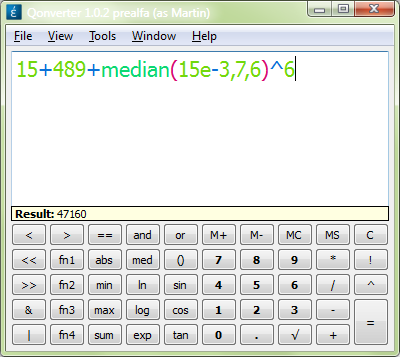
\includegraphics[width=7cm]{graphics/real-world/00-qon-native}
\caption{Native skin}
\end{subfigure}
~
\begin{subfigure}[b]{0.48\textwidth}
\centering
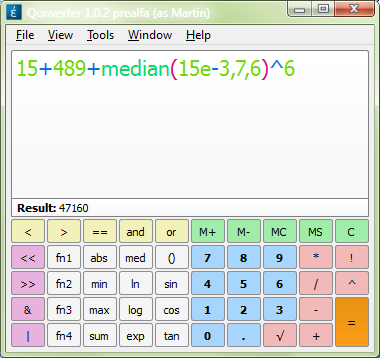
\includegraphics[width=7cm]{graphics/real-world/00-qon-modern}
\caption{Modern skin}
\end{subfigure}
\caption{Skinned Qonverter}\label{figure:skinsq}
\end{figure}

\subsection{Tray icon and desktop integration}
Desktop applications can be divided into two groups:
\begin{enumerate}
\item Applications which are executed manually if needed. They are closed after usage.
\item Applications which run constantly. They can be hidden (typically) into notification area of a desktop environment.
\end{enumerate}

We probably use some applications very rarely, so they don't need to run all the time. We simply open them, do needed job and then close them. It's sometimes better to keep certain applications in main memory and hidden so that they don't disturb us. Tray icon is amazing tool to achieve that. This is typical for applications which are used regularly.

Qonverter supports both modes. If we want to use it irregularly and not too often, then Qonverter can run in single-window mode and quit if window gets closed. But if we are advanced users who use calculator often, then Qonverter can be hidden to a tray area and only a tray icon remains visible. Interaction with a tray icon is critical because its the only user interface element visible if application windows are hidden.

\subsubsection{Single-window mode}
This is the default mode for Qonverter. It is also used in desktop environments which don't support tray icon mode. This mode offers standard windows and dialogs. Qonverter exits when last window is closed by a user.

\subsubsection{Tray icon mode}
Tray icon mode (\autoref{figure:opttray}) offers greater functionality. We can use windows and dialogs again. But Qonverter doesn't have to (but can) quit if last window is closed. It can minimize itself into notification area, resulting in last visible element\,--\,the tray icon. User can switch between modes freely via configuration dialog (\autoref{figure:settingsgui}).

\begin{figure}[ht]
\begin{center}

\includegraphics[width=7cm]{graphics/real-world/01-tray.png}
\caption{Qonverter tray icon}\label{figure:opttray}
\end{center}
\end{figure}

\begin{figure}[ht]
\begin{center}
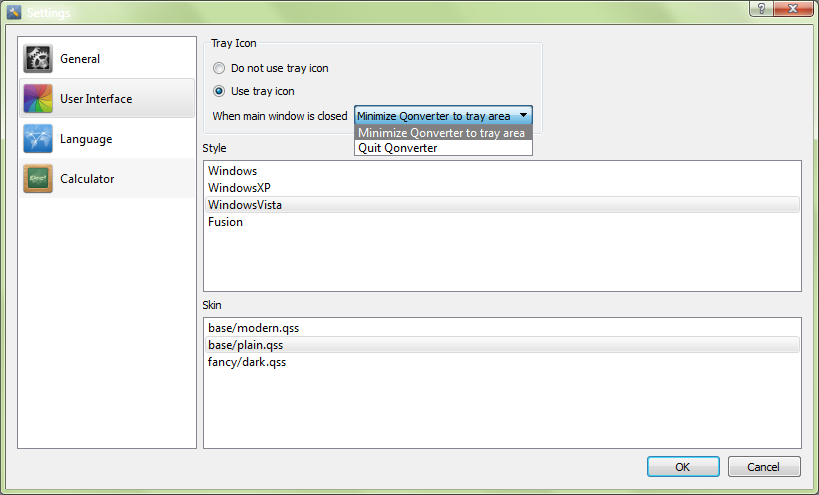
\includegraphics[width=13cm]{graphics/real-world/02-settings-gui.png}
\caption{Qonverter mode selection}\label{figure:settingsgui}
\end{center}
\end{figure}

\subsection{Displaying available functions, constants and variables}\label{chap:guii}
\fdocinlinecode{cpp}{!}{Calculator} class offers information about constats, variables and functions via\fdocinlinecode{cpp}{!}{ConstantsModel} class. It is used by functions/variables/constants overview dialog (see \autoref{figure:model1}). Model provides table-like data. Dialog uses\fdocinlinecode{cpp}{!}{ConstantsView} class to display those data.

\begin{figure}[ht]
\centering
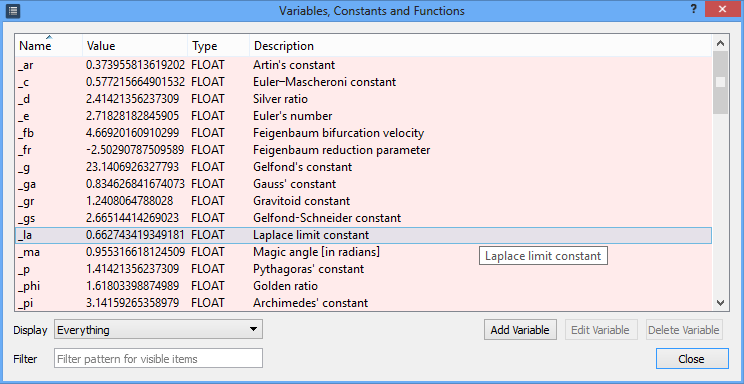
\includegraphics[width=13cm]{graphics/real-world/07-model1.png}
\caption{Dialog with overview of variables, constants and functions}\label{figure:model1}
\end{figure}

\subsection{Auto-completion}
Auto-completion (see \autoref{figure:autoq}) is known from advanced text editors or integrated development environments. It is usually displayed as a \enquote{floating} panel. User writes some text and auto-completion panel offers him available completions. This mechanism has use cases in calculator applications too. User doesn't have to remember names of built-in functions. Moreover, auto-completer can offer names of variables and constants.

\begin{figure}[ht]
\centering
\begin{subfigure}[t]{0.48\textwidth}
\centering
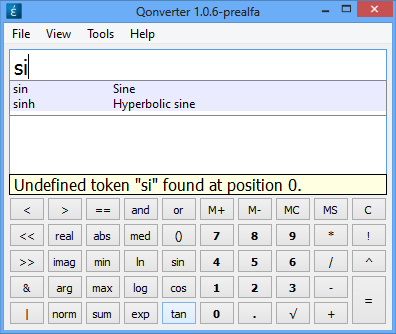
\includegraphics[width=7cm]{graphics/real-world/08-complete1.png}
\caption{Two functions in completion list}
\end{subfigure}
~
\begin{subfigure}[t]{0.48\textwidth}
\centering
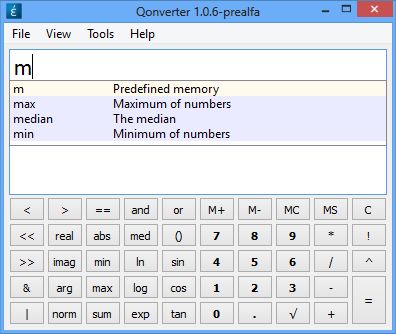
\includegraphics[width=7cm]{graphics/real-world/08-complete2.png}
\caption{Two functions and one variable in completion list}
\end{subfigure}
\caption{Auto-completion in Qonverter}\label{figure:autoq}
\end{figure}

\subsection{Unit and currency converter}
Unit converter doesn't contain special elements, except one thing. It doesn't contain single button for triggering a conversion. All conversions are done on-the-fly. User gets hints about what to do via placeholder texts of input controls (\autoref{figure:unit}).

\begin{figure}[ht]
\centering
\begin{subfigure}[b]{0.48\textwidth}
\centering
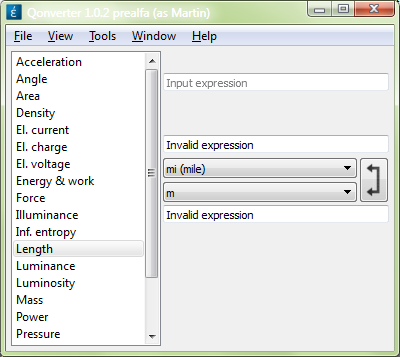
\includegraphics[width=7cm]{graphics/real-world/03-unit}
\caption{Initial state}
\end{subfigure}
~
\begin{subfigure}[b]{0.48\textwidth}
\centering
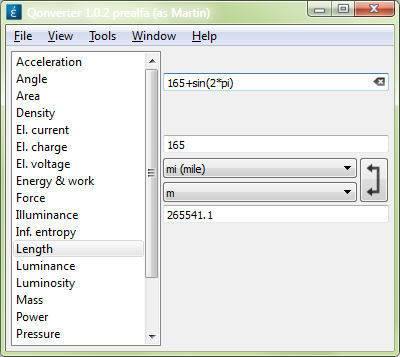
\includegraphics[width=7cm]{graphics/real-world/03-unit-full}
\caption{With calculated and converted value}
\end{subfigure}
\caption{Unit converter overview}\label{figure:unit}
\end{figure}